\chapter{Konzept} \label{chap:Konzept}
In diesem Kapitel soll das Konzept dieser Ausarbeitung vorgestellt werden. Dieses besteht aus vier Teilen. Zuerst soll das Vorgehen erklärt werden, gefolgt von der Darstellung des Environments und der Agenten. Danach soll im weiteren auf die Datenerhebung eingegangen werden.\\
Ziel dieses Abschnittes ist es, das Vorgehen und alle weiteren dazu benötigten Elemente unabhängig von der Implementierung darzustellen, sodass die Ergebnisse mit jeder universell reproduzierbar sind.

\section{Vorgehen} \label{sec:Konzept_Vorgehen}
Das Vorgehen lässt sich am besten mit Hilfe eines Flussdiagramms darstellen, in welchem die einzelnen Schritte des Vergleichs visuell dargestellt werden.\\
Zu Beginn sei erwähnt, dass die Annahme getroffen wird, dass alle für die Vergleiche benötigten Komponenten, wie z.B. Environment, Agenten und statistische Analysekomponenten, entsprechende der Anforderungen implementiert sind (siehe \ref{chap:Anforderungen}).\\
Als erstes werden die Agenten erstellt (siehe \ref{fig:Vorgehen}). Für diese diesen Zweck werden mehrere Klassen mit verschiedenen Hyperparametern generiert bzw. ausgewählt.
Mit dieser Baseline-Agenten-Menge werden nun die weiteren Vergleiche durchgeführt.\\
Zu Beginn werden für jedes Evaluationskriterien die zwei optimalsten Baseline Agenten bestimmt. Auf diese sollen die Optimierungen angewendet werden. 
Aufgrund der Tatsache, dass das Anwenden der Optimierungen viel Zeit und Ressourcen bindet, sollen diese nur auf die vielversprechendsten Agenten angewendet werden. Dies führt zu einer Konvergenz des Verfahrens.\\
Der verwendete Algorithmus besitzt dabei keinen Einfluss auf die Auswahl der Agenten, sodass auch zwei DQN oder PPO Agenten optimiert werden können. Genauere Details zur Durchführung der Baseline Vergleiche finden sich im Abschnitt \ref{sec:Konzept_Datenerhebung}.\\
Basierend auf den beiden Sieger Agenten (Baseline Winner Agent-01 und Baseline Winner Agent-02) der Baseline Vergleiche (siehe \ref{fig:Vorgehen}), werden nun die Optimierungen angewendet. Mit diesen optimierten Agenten (Agent-01 Optimierung A bis Agent-02 Optimierung B) werden nun die Vergleiche bezüglich jedes einzelnen Evaluationskriteriums \ref{tab:Kriterien} erneut wiederholt.\\
Im letzten Schritt soll in der gesamt Evaluation der optimale Agent für jedes Evaluationskriterium ermittelt werden. Dabei können dies auch Baseline Agenten sein. Es ist nicht zwingend zugesichert das optimierte Agenten die optimalsten dies.
\begin{figure}[H]
	\centering
	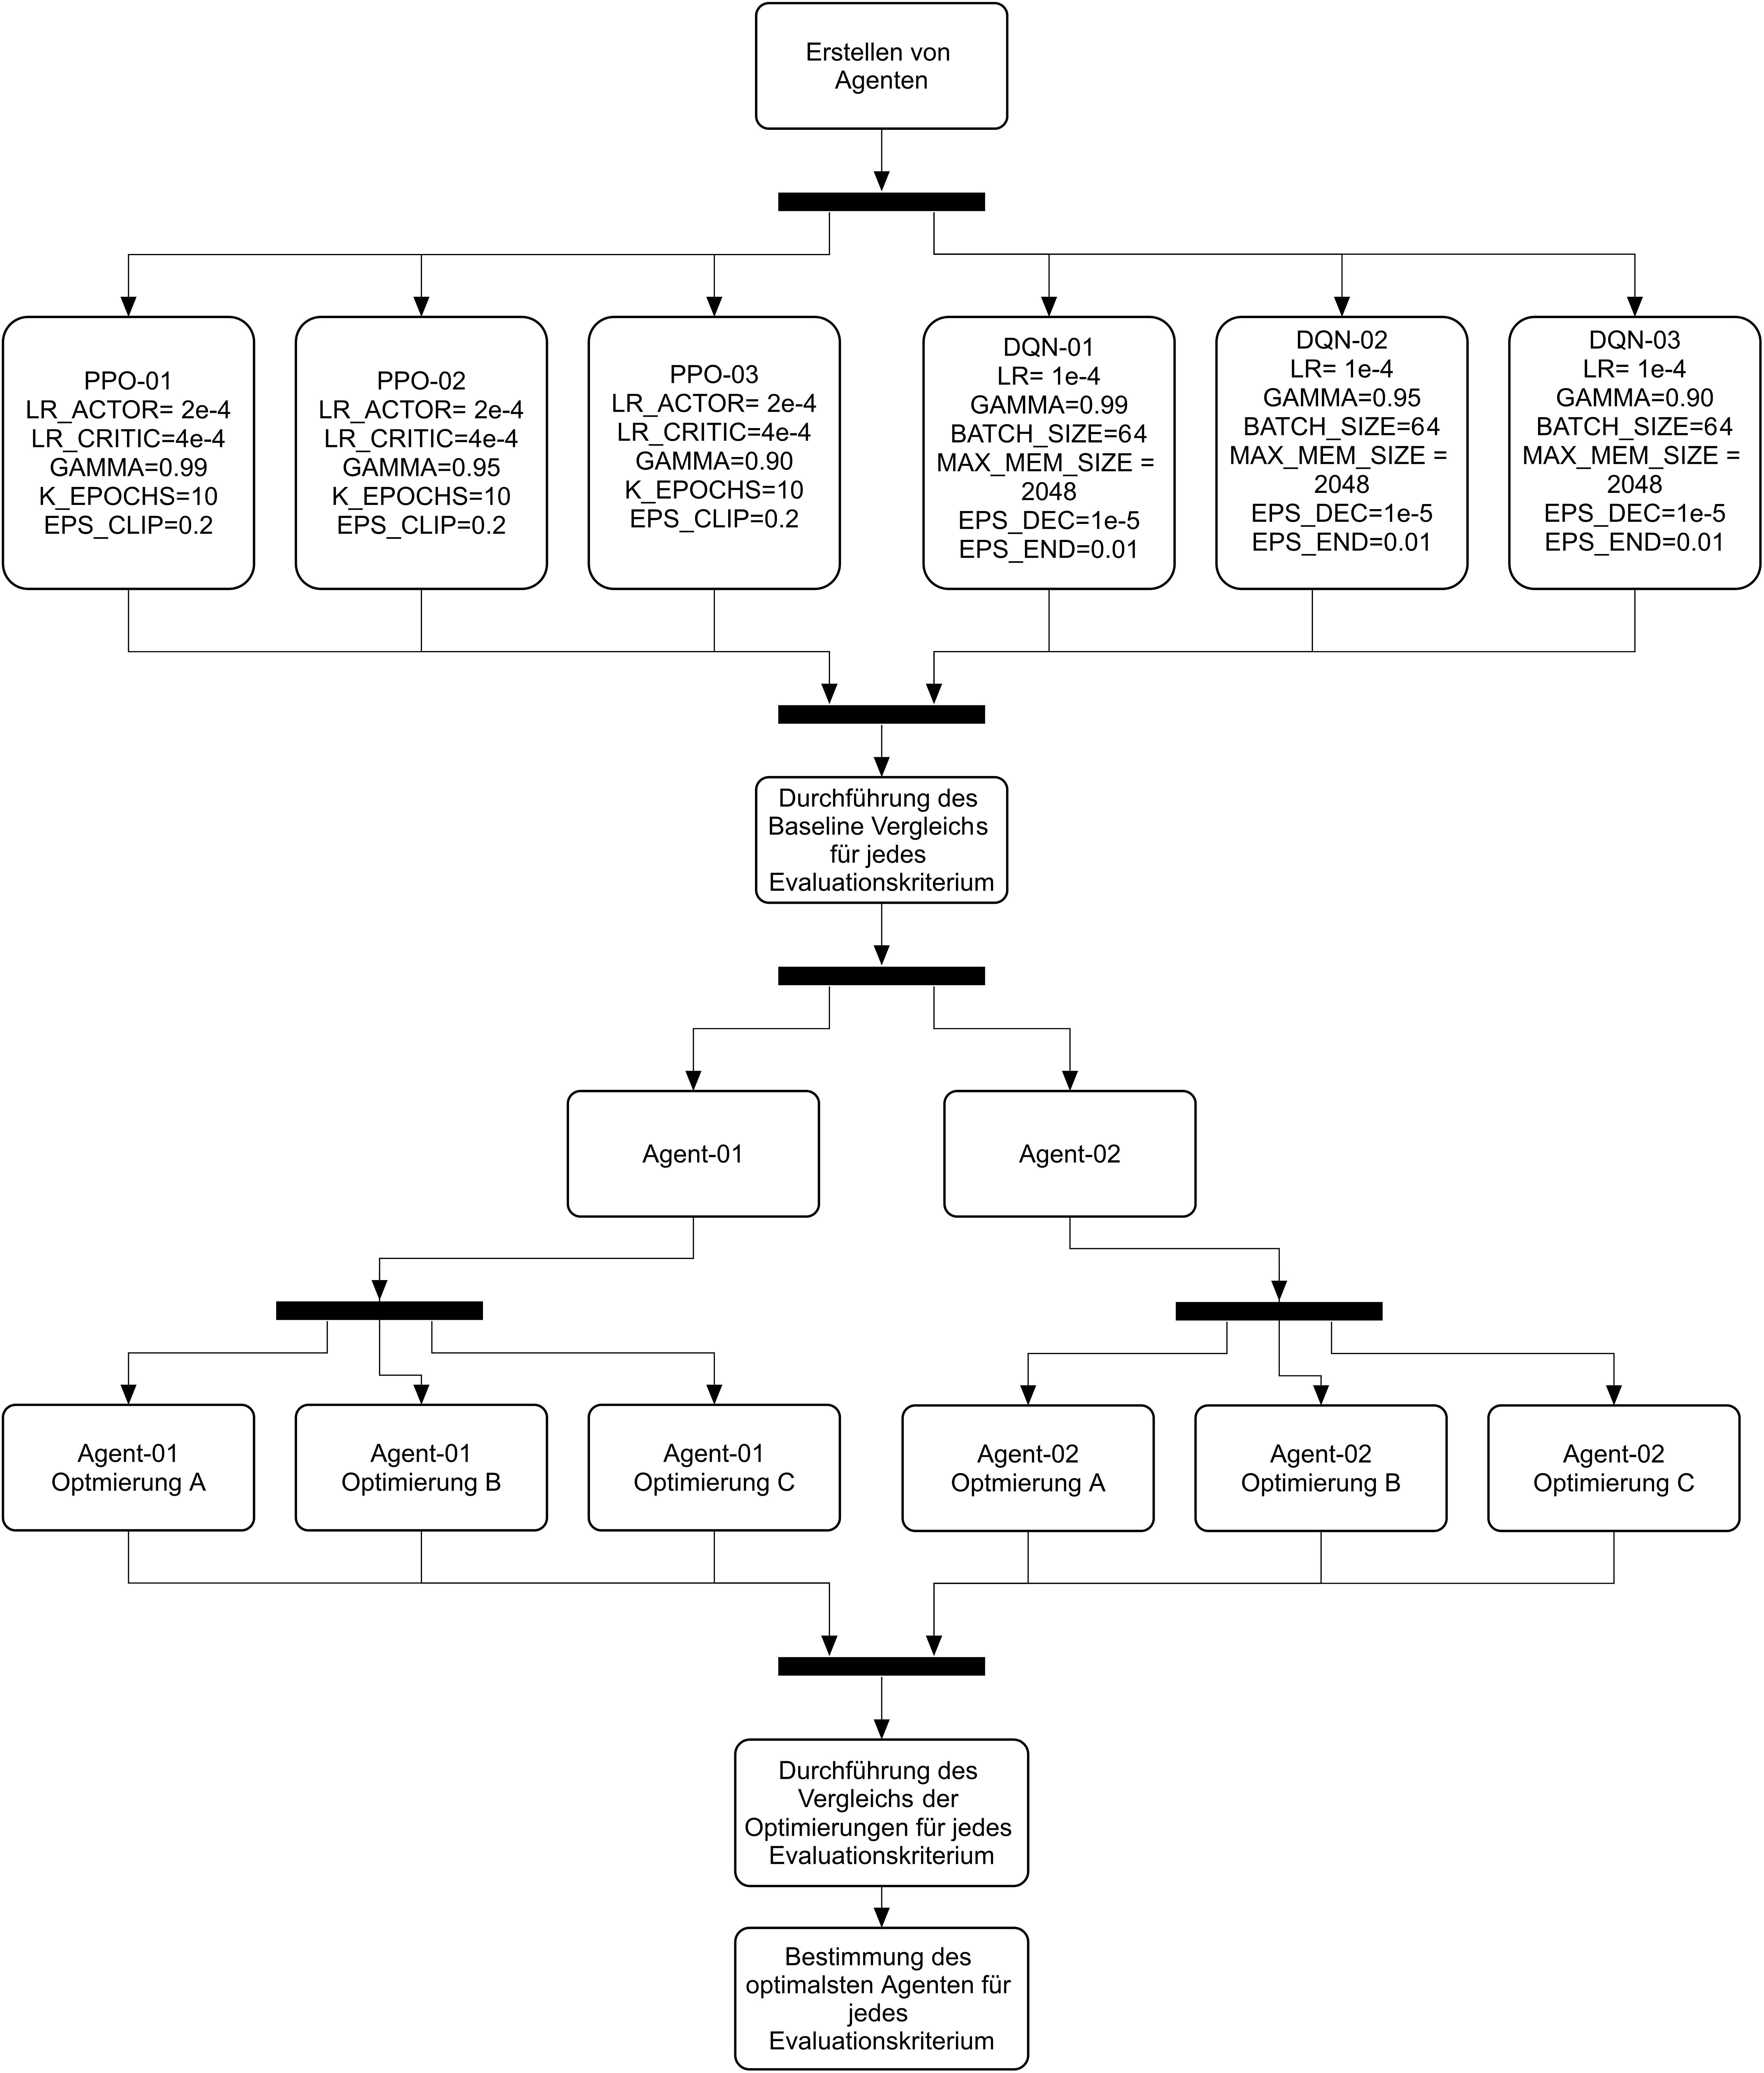
\includegraphics[scale=0.095]{Abbildungen/Vorgehen.png}
	\caption[Flussdiagramm des Vorgehens]{Darstellung des Vorgehens.}
	\label{fig:Vorgehen}
\end{figure}

\section{Environment} \label{sec:Konzept_Environment}
Das Env besteht im wesentlichen aus einer Hauptkomponenten, der Spiellogik, welche von einer Schnittstellen-Komponente umschlossen wird. Diese soll mit einer standardisierten Schnittstelle (siehe \ref{sec:Anforderungen_Schnittstelle}) implementiert werden.\\
Die Spiellogik kapselt die Game-, Player-, Reward-, Observation- und GUI-Komponenten, welche im Folgenden näher erklärt werden.

\subsection{Spiellogik} \label{sec:Konzept_Spiellogik}
Die Spiellogik besteht aus den fünf Unterkomponenten, welche in \ref{sec:Konzept_Environment} bereits benannt wurden.\\
Die Game-Komponente stellt die Hauptkomponente dar, da sie die eigentliche Aktionsdurchführung implementiert. Sie beinhaltet jeweils Instanzen der Reward-, Observation-, GUI- und Player-Komponenten. Letztere ist eine Datenhaltungskomponente, welche die Daten der Snake, wie z.B. Position oder Ausrichtung (direction) beinhaltet.\\
\\Die Reward-Komponente bestimmt den auszugebenden Reward nach jeder Aktionsabfertigung. Dieser berechnet sich wie in \ref{sec:Konzept_Reward} angegeben. Zuzüglich wird im Rahmen der Optimierungen A, (siehe \ref{sec:Konzept_Optimierung01}), eine weitere Reward Funktion implementiert.\\
\\In der Game-Komponente werden wichtige Spielbezogene Daten verwaltet. Zu diesen gehören das Spielfeld (ground), sowie die Form des Spielfeldes (shape) und die Position des Apfels auf dem Spielfeld. Sie beinhaltet viele Methoden, wie z.B. die action, observe, evaluate, reset und view Methode.\\
\\In der Player-Komponente werden Spielerbezogene Daten verwaltet. Zu diesen zählen die Position des Kopfes der Snake, sowie ihrer Schwanzglieder, ihre Ausrichtung (direction), ihre gelaufenen Schritte seit dem letzten Fressen eines Apfels (inter\_apple\_steps), ihr Lebensstatus (is\_terminal), daher ob sie tot oder lebendig ist und weitere Farbkonstanten für die GUI.\\
\\Die Observation-Komponente beinhaltet viele einzelne Funktionen zur schrittweisen Erstellung der Observation, wie sie in Abschnitt \ref{sec:Konzept_Observation} erklärt wird.\\
\\Zur Erzeugung der grafischen Oberfläche implementiert die GUI-Komponente die Funktionalität ein Fenster zu öffnen, welches das Spielgeschehen, daher das Spielfeld (ground), anzeigt und stetig an den neusten Stand anpasst.
\begin{figure}[H]
	\centering
	\def\svgscale{0.17}
	\input{Abbildungen/Spiellogik.pdf_tex}
	\caption[Spiellogik]{Darstellung der Spiellogik mit ihren Unterkomponenten.}
	\label{fig:Spiellogik}
\end{figure}

\subsubsection{Spielablauf} \label{sec:Konzept_Spielablauf}
Die eigentliche Aktionsabarbeitung wird durch das Aufrufen der step Funktionalität in der Schnittstellen-Komponente (siehe \ref{sec:Konzept_Schnittstelle}) bewirkt. Diese ruft die evaluate und observe Methoden auf, welche in der Game-Komponente implementiert sind (siehe \ref{fig:Spiellogik}).
Um jedoch die Abarbeitung einer Aktion durchzuführen, muss zuerst die action Methode aufgerufen werden, welche die von Agenten bestimmte Aktion übergeben bekommt. 
\begin{figure}[H]
	\centering
	\def\svgscale{0.089}
	\input{Abbildungen/Spielablauf.pdf_tex}
	\caption[Spielablauf]{Darstellung eines Schrittes in der Spielepisode.}
	\label{fig:Spielablauf}
\end{figure}
Zu Beginn wird überprüft, ob die Snake seit dem letzten Fressen mehr Schritte als die eigentliche Spielfeldgröße gegangen ist. Diese berechnet sich dabei aus der Spielfeldform (shape). Normal liegt diese bei 64. Im Rahmen der Bestimmung der Robustheit, wird sich diese im Testverlauf jedoch noch ändern (siehe \ref{sec:Konzept_Datenerhebung}).\\
Sollte die Snake mehr Schritte gelaufen sein als die Größe des Spielfelds, so wird das Spiel terminiert, da die Snake eventuell in einer Schleife steckt.\\
Andernfalls wird die Aktion verarbeitet, indem sie die Ausrichtung (direction) der Snake manipuliert. Das Spiel Snake besitzt in diesem Konzept drei Aktionen: turn left, turn right oder do nothing.
\begin{longtable}[h]{|p{4cm}|p{\linewidth - 5cm}|}
	\caption{Kodierung der Aktionen}
	\label{tab:Aktionscodierung} 
	\endfirsthead
	\endhead
	\hline
	Aktion & Erklärung \\
	\hline
	turn left & Die Snake ändert ihre Richtung um 90° nach links. Z.B. Von N $\longrightarrow$ W \\
	\hline
	turn right & Snake ändert ihre Richtung um 90° nach rechts. Z.B. Von N $\longrightarrow$ O \\
	\hline
	do nothing & Die Richtung der Snake wird nicht verändert. \\
	\hline
\end{longtable}
Entsprechend der Beispiele in Tabelle \ref{tab:Aktionscodierung} wird klar, dass die Ausrichtung (direction) entweder nur Norden, Osten, Süden oder Westen sein kann.
Als nächstes wird ein Schritt der Snake mit der aktualisierten Ausrichtung hypothetisch durchgeführt. Dabei lässt sich feststellen, ob die Ausführung des Schrittes zum Tod der Snake führt. Sollte dies der Fall sein, so wird der Spielablauf terminiert. Dabei führt das Laufen in sich selbst und das Verlassen des Spielfeldes zum Tod (siehe \ref{sec:Snake}).\\ 
Anderenfalls wird der Schritt durchgeführt. Dabei wird zwischen zwei Fällen unterschieden.\\
Sollte die Snake einen Apfel gefressen haben, also Kopf und Apfel die selbe Position einnehmen, so wächst die Snake um ein Schwanzglied. Der alte Apfel wird entfernt und ein neuer erscheint zufallsbasiert irgendwo auf einem freien Feld des Spielfelds.\\
Sollte die Snake hingegen keinen Apfel gefressen haben, so geht sie einfach den Schritt, es bewegen sich daher alle Schwanzglieder auf die Vorgängerposition, mit Ausnahme des Kopfes, welcher die neue Position einnimmt.\\
Nach der Ausführung einer dieser beiden Fälle, wird die GUI mit der update\_gui Methode aktualisiert. Nach diesem Schritt ist die Abarbeitung der action Methode abgeschlossen.\\
Damit jedoch der Agent den Nachfolgezustand und Reward erhält, wird die evaluate Methode in der Reward-Komponente und die observe Methode in der Observation-Komponente aufgerufen.
Zum Schluss werden Obs und Reward zurückgegeben.

\subsubsection{Reward} \label{sec:Konzept_Reward}
Die evaluate Methode befindet sich in der Game-Komponente und ruft ihrerseits die standard\_reward Methode in der Reward-Komponente auf. Sie bestimmt, basierend auf dem letzten Zug, den Reward. Dies geschieht nach dem folgenden Vorbild.
Der Standard Reward ist abhängig von drei Faktoren. Dem Fressen eines Apfels, dem Sieg oder dem Verlust. Sollte keiner dieser genannten Faktoren eintreten, wird ein Reward von -0.01 zurückgegeben. Dies hält den Agenten dazu an den kürzesten Pfad zum Apfel zu finden, da jeder Schritt geringfügig bestraft wird.\\
War es der Snake möglich einen Apfel zu fressen, so wird ein Reward von +2.5 zurückgegeben, da ein Sub-Goal erfüllt worden ist.
Sollte die Snake gestorben sein, durch das Verlassen des Spielfeldes oder das Laufen in sich selbst oder das zu lange Umherlaufen, so wird ein Reward von -10 zurückgegeben, um dieses Verhalten in seiner Häufigkeit zu minimieren.
Hat die Snake alle Äpfel gefressen, sodass das gesamte Spielfeld mit der Snake ausgefüllt ist, so wird ein Reward von +10 zurückgegeben, um ein solches Verhalten in seiner Häufigkeit zu maximieren. Dies Snake hat zu diesem Zeitpunkt dann das Spiel gewonnen.\\
Die zweite Reward Funktion wird im Rahmen der Optimierung A (siehe \ref{sec:Konzept_Optimierung01}) näher erklärt.

\subsubsection{Observation} \label{sec:Konzept_Observation}
Die Observation, welche von der step Methode der Schnittstellen-Komponente (siehe \ref{sec:Konzept_Schnittstelle}) zurückgegeben wird, besteht aus der around\_view (AV) und der scalar\_obs (SO). Zur Erstellung der Obs wird die observe Methode in der Game-Komponente (siehe \ref{sec:Konzept_Spiellogik}) aufgerufen. Diese ruft wiederum ihrerseits die make\_obs Funktion in der Observation-Komponente auf. Mit Hilfe verschiedener Unterfunktionen wird dann die Obs generiert.\\
Die AV lässt sich dabei als ein Ausschnitt des Spielfeldes (ground) beschreiben, welcher einen festen Bereich um den Kopf der Snake abdeckt.
Strukturen wie Wände und Teile des eigenen Schwanzes, welche vielleicht eine Sackgasse aufspannen könnte, werden dadurch deutlich. Mathematisch ist die AV eine one-hot-encoded Matrix der Form (6x13x13).\\
\\Das One-Hot-Encoding ist ein binäres encoding System. Sollte ein Merkmal vorhanden sein, so wird dieses mit eins codiert anderenfalls mit null. \cite[S. 359 f.]{DRL_Lapan}\\
Dies ist auch der Grund, warum die AV Matrix sechs Channel (zweidimensionale Schichten) besitzt. Diese geben Aufschluss über folgende Informationen:
\begin{longtable}[h]{|p{4cm}|p{\linewidth - 5cm}|}
	\caption{Channel-Erklärung der Around\_View (AV)}
	\label{tab:around_view} 
	\endfirsthead
	\endhead
	\hline
	Channel der Matrix bzw. Erste Dimension (Ax13x13) & Erklärung \\
	\hline
	A = 0 & Die erste Feature Map signalisiert den Raum außerhalb des Spielfelds. Nährt sich die Snake dem Rand, so würde der Ausschnitt der AV aus dem Spielfeld herausragen und den Eindruck erwecken, dass dieses größer wäre als es in Realität wirklich ist. Darum werden Felder der AV, die sich außerhalb des Spielfelds befinden, angezeigt.\\
	\hline
	A = 1 & Diese Feature Map stellt alle Schwanzglieder mit Ausnahme des Kopfes und es letzten Schwanzgliedes dar. \\
	\hline
	A = 2 & In dieser Feature Map wird der Kopf der Snake dargestellt. \\
	\hline
	A = 3 & Damit gegen Ende des Spiels der Agent noch freie Felder erkennen kann, wird in dieser Feature Map jedes freie und sich im Spielfeld befindliche Feld mit eins codiert. \\
	\hline
	A = 4 & Die vorletzte Feature Map codiert das Schwanzende der Snake. \\
	\hline
	A = 5 & In der letzte Feature Map wird der Apfel abgebildet. \\
	\hline
\end{longtable}
Vorteilhaft an der AV ist, dass, im Gegensatz zu den Obs in den verwandten Arbeiten \cite{Autonomous_Agents_in_Snake_Game_via_DRL} und \cite{UAV}, nicht das gesamte Feld übertragen wird, sondern nur der wichtigste Ausschnitt, was die Menge an zu verarbeiten Daten reduziert. Des Weiteren ergeben sich keine Probleme zwischen variablen Spielfeldgrößen und der Input-Size von Convolutional Layers (siehe \ref{sec:Anhang_Conv_Layer}).\\
Ein Nachteil dieser Obs ist jedoch die Unvollständigkeit. Sollte der blaue Punkt (der Apfel) in Abbildung \ref{fig:Observation} außerhalb des grauen Kasten und daher außerhalb der AV liegen, so bleibt der Agent im Unklaren über den Aufenthaltsort des Apfels.
Auch Informationen wie z.B. der Hunger, also die verbleibenden Schritte bis das Spiel endet, Distanzen zu den Wänden und Schwanzteilen und die Ausrichtung (direction) der Snake, werden durch die AV nur eingeschränkt oder gar nicht geliefert.
\begin{figure}[H]
	\centering
	\def\svgscale{0.80}
	\input{Abbildungen/Observation.pdf_tex}
	\caption[Observation]{Partielle Darstellung der verwendeten Observation. Das blaue Rechteck und dessen Schwanz stellt die Snake dar, wobei das rot umrandete Rechteck den Kopf darstellt. Die schwarzen Felder werden nicht von der AV abgedeckt, graue liegen innerhalb der AV. 
		Die gelben gestrichelten Linien stellen eine Raytracing Distanzbestimmung dar. Der blaue Kreis stellt den Apfel dar und der grüne viertel Kreis oben links symbolisiert den Hunger.}
	\label{fig:Observation}
\end{figure}
Aus diesem Grund wurde die AV durch die scalar\_obs (SO) ergänzt.
Die SO beinhaltet skalare Informationen und ist eine Konkatenation aus Raytracing Distanzbestimmung, Hunger- und Blickrichtungsanzeige (direction). Zuzüglich werden der SO noch zwei Kompasse für relative Positionsinformation zwischen Kopf und Apfel bzw. letztem Schwanzglied hinzugefügt.\\
Letztere sind eindimensionale Vektoren, welche über das One-Hot-Encoding anzeigen, ob sich das gesucht Objekt relativ zum Kopf oberhalb, unterhalb oder in der selben Zeile befindet (Matrixsicht). Analog verhält es sich mit der vertikalen Sicht.\\
Die Blickfeldanzeige ist ebenfalls one-hot-encoded und stellt mit ihrem Vektor die vier Ausrichtungen Norden, Osten, Süden und Westen dar.\\
Der Hunger ist die Differenz zwischen der Anzahl der gegangenen Schritten seit dem letzten Fressen (inter\_apple\_steps) und der maximalen Schrittanzahl (max\_steps). Diese maximale Schrittanzahl ist als Spielfeldgröße definiert. Da der Hunger bei einer großen Differenz einen kleinen Einfluss und bei einer geringen Differenz einen großen Einfluss besitzen soll, wurde dieser durch eins geteilt. Nähren sich die beiden Werte im Nenner an, so rückt der gesamt Wert des Bruches näher an unendlich, da den Nenner immer kleiner wird.
\begin{align}
	\min(2, \frac{1}{inter\_apple\_steps - max\_steps})
\end{align}
Um mit der Unendlichkeit auftretende Probleme zu umgehen wird zwei zurückgegeben, wenn die Differenz null ist.\\
In ähnlicher Weise wird mit den Raytracing Distanzbestimmungen verfahren. Bei ihnen handelt es sich um acht Distanzmesserlinien, die in 45° Abständen ausgesandt werden, siehe Abbildung \ref{fig:Observation}. Befindet sich das gesucht Objekt in dieser Linie, so wird die Distanz zwischen dem Kopf der Snake und dem Objekt durch eins dividiert und zurückgegeben. Es wird dabei nach Wänden, dem eigenem Schwanz und dem Apfel gesucht. Daher wird die Raytracing Distanzbestimmung in einem Vektor der Größe 24 (3 * 8 = 24) gespeichert.

\subsubsection{GUI}
Die graphische Oberfläche oder auch GUI genannt kann optional ein- oder ausgeschaltet werden. Beim Lernen der Agenten bietet es sich beispielsweise an diese auszuschalten, da diese die Lerngeschwindigkeit senkt. Beim Start der GUI wird ein Fenster geöffnet, welches den momentanen Stand der Spielgeschehens anzeigt. Da Snake eine zweidimensionale Spieloberfläche besitzt, wird diese im Fenster dargestellt. Nach jeder Aktionsdurchführung muss die GUI mit der update\_gui Methode aktualisiert werden, um stets den neusten Stand des Spiels zu zeigen.

\subsection{Schnittstelle} \label{sec:Konzept_Schnittstelle}
Die Schnittstelle umschließt die bereits erwähnte Spiellogik-Komponente mit ihren Unterkomponenten, um eine standardisierte Schnittstelle zu erzeugen.
\begin{figure}[H]
	\centering
	\def\svgscale{0.15}
	\input{Abbildungen/Wrapper.pdf_tex}
	\caption[Schnittstelle]{Darstellung der Schnittstelle.}
	\label{fig:Schnittstelle}
\end{figure}
Die step Funktionalität (siehe \ref{fig:Schnittstelle}) stellt die Hauptmethode der Schnittstellen-Komponente dar. Sie bekommt eine Aktion übergeben, welche zuvor von einem Agenten bestimmt wurde. Diese wird mit Hilfe der Spiellogik umgesetzt. Entsprechend der Anforderung der Standardisierte Schnittstelle (siehe \ref{sec:Anforderungen_Schnittstelle}) gibt diese Methode nur Reward und Observation zurück.\\
Reset setzt den bereits vorhandenen Spielfortschritt zurück, wobei die reset Methode der Game-Komponente aufgerufen wird. Dies soll entsprechend der Reset Anforderung (siehe \ref{sec:Anforderung_Reset}) geschehen.\\
Die Render Methode ist für die Visualisierung verantwortlich und ruft die update\_gui Methode in der GUI-Unterkomponente auf, welche das Spielfeld, entsprechend der Render Anforderung (siehe \ref{sec:visualisierung_Env}) graphisch darstellt.\\
Die has\_won und has\_ended Methoden geben Statusinformationen über den momentanen Spielstand zurück, welche für die Test- und Trainingsabläufe benötigt werden.

\newpage
\section{Agenten} \label{sec:Konzept_Agenten}
In diesem Abschnitt des Konzepts sollen die Agenten inklusive ihrer Netzstruktur vorgestellt werden. Zu diesem Zweck müssen die Algorithmen (DQN und PPO) näher beleuchtet werden.

\subsection{Netzstruktur} \label{sec:Konzept_Netzstruktur}
Zu Beginn soll die Netzstruktur erklärt werden, wobei dies unabhängig von den Algorithmen geschehen kann, da sowohl DQN als auch PPO Agenten das annähernd gleiche Netz nutzen.

\begin{wrapfigure}{r}{5cm}
	\centering
	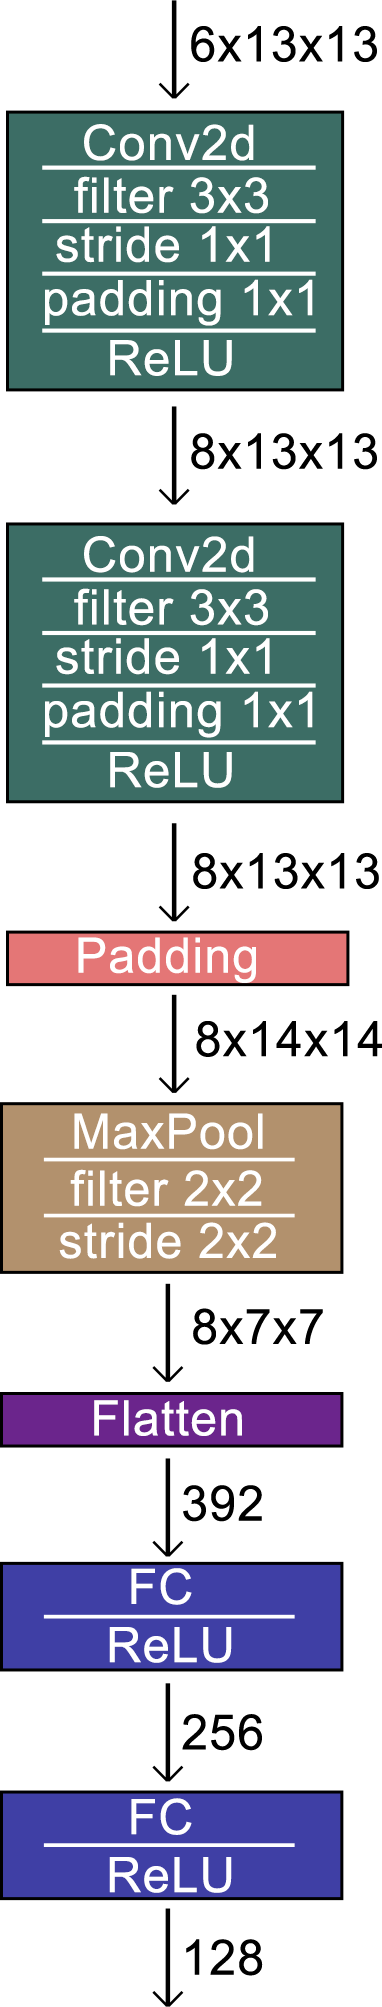
\includegraphics[width=3.0cm, height=15.5cm]{Abbildungen/ConvNet.png}
	\caption[AV-Network]{\\AV-Network}
	\label{fig:AV-Network}
\end{wrapfigure}

Im Rahmen dieser Ausarbeitung soll sich nur auf eine Netzstruktur konzentriert werden, um die Vergleichbarkeit der einzelnen Algorithmen zu erhöhen. Dennoch müssen, aufgrund des Algorithmus, kleinere Anpassungen an der Netzstruktur vorgenommen werden. Diese werden im Weiteren erklärt.\\
Dieses NN stellt dabei einen Kompromiss zwischen Vollständigkeit und Effizienz dar. In den Papers von \cite{Autonomous_Agents_in_Snake_Game_via_DRL} und \cite{UAV} wurden nur großes CNN (siehe \ref{sec:Anhang_CNN}) genutzt, die Gefahr laufen viele unnötige Informationen verarbeiten zu müssen. Zusätzlich können noch Probleme mit variablen Spielfeldgrößen auftreten, sodass in dieser Ausarbeitung auf ein zweiteilige Netzstruktur gesetzt wird. Diese besteht aus dem AV-Network und dem Actor-, Critic- oder Q-Tail.
Zuerst wird die AV durch das AV-Network geleitet. 
Dabei wird die AV durch zwei Convolutional Layer mit einer ReLU Aktivierungsfunktion propagiert. Dabei erhöht sich die Channel-Anzahl auf acht, wobei eine weitere Erhöhung der Channel-Anzahl aufgrund der bereits sehr stark optimierten AV nicht nötig ist. Die Feature Map wird während dieses Prozesses nicht minimiert, aufgrund des Paddings der Convolutional Layers. Dies soll den Informationsverlust an den Rändern minimieren.\\  
Danach werden allen Feature Maps eine Null-Zeile und Null-Spalte hinzugefügt (Padding), damit beim Max-Pooling, unter der Filtergröße und dem Stride von 2x2, auch die letzten Zeile und Spalte verarbeitet werden. Der Tensor besitzt nun die Form (8x14x14). Nach dem max-pooling besitzen die Feature Maps jedoch nur noch eine Größe 7x7 (Tensor: 8x7x7).\\ 
Dann folgt die Einebnung (Flatten) zu einem eindimensionalen Tensor, welcher daraufhin durch zwei weitere Fully Connected Layer (FC) mit einer ReLU Aktivierungsfunktion propagiert wird. Der resultierende Tensor besitzt die Größe 1x128 und ist ein Zwischenergebnis, da dieser nun mit der SO verbunden wird (Join). Der Vorgang ist in der Abbildung \ref{fig:AV-Network} dargestellt.
%eine zeile platz sonst failed die Formartierung
\begin{wrapfigure}{l}{5.1cm}
	\centering
	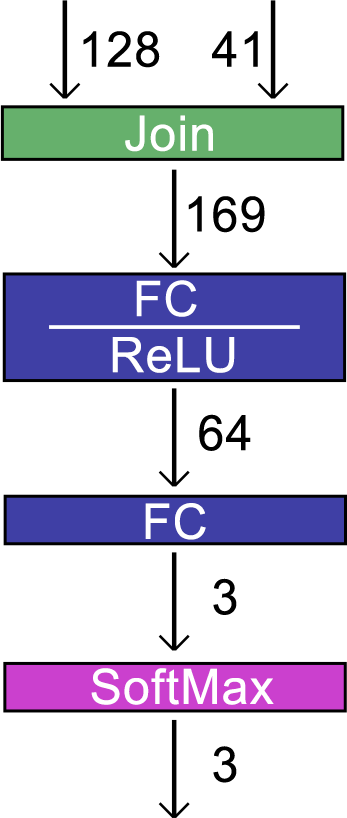
\includegraphics[width=3.0cm, height=8.0cm]{Abbildungen/Actor.png}
	\caption[Actor-Head]{\\Actor-Tail}
	\label{fig:Actor_Tail}
\end{wrapfigure}

Da das NN in beide Algorithmen verwendet wird, müssen Netzwerkschwänze für den Actor, Critic und für das Q-Network (Q-Net) definiert werden. Alle unterscheiden sich jedoch nur in ihrer Ausgabe. 
Nachdem der Joined Tensor (1x169), welcher aus dem Zwischenergebnis des AV-Networks und der SO besteht, durch zwei weitere FC Layer mit ReLU Aktivierungsfunktion propagiert wurde, benötigt der Actor des PPO Algorithmus eine Wahrscheinlichkeitsverteilung über alle Aktionen. Daher auch die Ausgabe von einem Tensor der Größe drei. Um diese Wahrscheinlichkeitsverteilung zu erhalten, wird die SoftMax Funktion angewendet, siehe Abbildung \ref{fig:Actor_Tail}.\\
Der Critic des PPO Algorithmus verwendet hingegen den Critic-Tail, siehe Abbildung \ref{fig:Critic_Q_Tail} links. Dieser leitet den Joined Tensor durch ein weiteres FC Layer mit ReLU Aktivierung. Der Resultierende Output wird danach durch ein weiteres FC Layer ohne Aktivierung geleitet. Da der Critic für jeden State die Discounted Sum of Rewards bestimmt (siehe \ref{sec:Baseline_Estimate}), gibt dieser einen Tensor mit einem einzigen Wert zurück (Skalar).
Der Q-Net-Tail ist in seinem Aufbau sehr ähnlich zum Critic-Tail. Da dieser jedoch die Q-Values für jede Aktion im Zustand angeben soll, muss ein Tensor der Größe drei zurückgegeben werden. Von der Struktur des Netzes sind jedoch der Critic- und Q-Net-Tail, mit Ausnahme der Ausgabeschicht, gleich (siehe \ref{fig:Critic_Q_Tail}).
\begin{figure}[H]
	\centering
	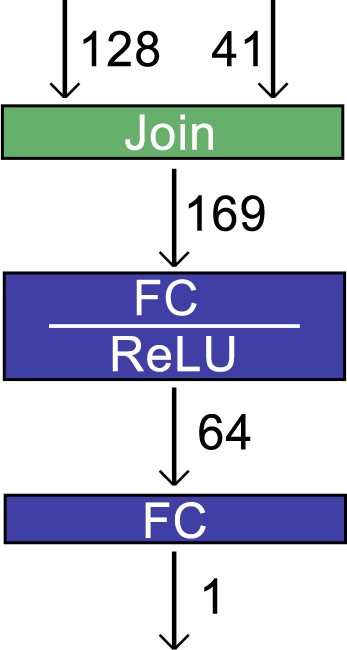
\includegraphics[width=3cm, height=5.2cm]{Abbildungen/Critic.png}
	\hspace{.3\linewidth}% Abstand zwischen Bilder
	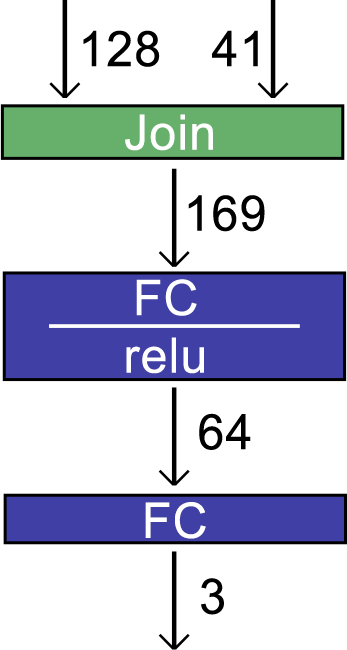
\includegraphics[width=3cm, height=5.2cm]{Abbildungen/QNet.png}
	\caption[Critic- und Q-Net-Tail]{Darstellung des Critic-Tail (links) und des Q-Net-Tail (rechts).}
	\label{fig:Critic_Q_Tail}
\end{figure}

\subsection{DQN} \label{sec:Konzept_DQN}
Der DQN Algorithmus und damit auch die Agenten, welche auf diesem basieren, bestehen aus drei Komponenten. Diese ermöglichen die Implementierung der Hauptmethoden act und learn.
\begin{figure}[H]
	\centering
	\def\svgscale{0.18}
	\input{Abbildungen/DQN-Agent.pdf_tex}
	\caption[DQN-Agent]{Darstellung des DQN-Agent mit seinen Komponenten.}
	\label{fig:DQN-Agent}
\end{figure}
Diese Hauptmethoden sind in der DQN-Komponente eingebettet, welche die zentrale Instanz des DQN darstellt. In ihr werden zudem die Memory und Q-Network Komponente verwaltet. Des Weiteren werden wichtige Konstanten für den DQN Algorithmus, wie z.B. Gamma, Epsilon (eps), Epsilon-Dekrementierung (eps\_dec), der minimal Wert für Epsilon (eps\_min), die Batch-Size (batch\_size), die maximale Größe des Memory (max\_mem\_size) und die Lernrate (lr), in der DQN-Komponente gespeichert.\\
Die Memory-Komponente speichert die gesammelten Erfahrungen des DQN-Agenten in einer Ring-Buffer Struktur. Sollte dieser Buffer voll sein, so werden die ältesten Erfahrungen, welche am Anfang stehen, mit den neuen überschrieben.
Die gespeicherten Erfahrungen werden im weiteren Verlauf von der learn Methode abgerufen, um mit ihnen den Lernprozess durchzuführen. 
Abzuspeichernde Werte, für jeden Schritt, sind dabei die around\_view (AV), die scalar\_obs (SO) die Aktion (action), der Reward (reward), die Information, ob man sich in einem terminalen Zustand befindet (terminal) und die around\_view (AV\_) und scalar\_obs (SO\_) des Nachfolgezustandes.\\
Die Q-Network-Komponente verwaltet das NN (Q-Network). Dieses wird von den act Methoden dazu genutzt, um die Aktionen für das Env zu bestimmen. Des Weiteren wird das Q-Network durch die learn Methode aktualisiert, sodass eine höhere Performance erreicht werden kann.

\subsubsection{Aktionsauswahlprozess} \label{sec:Konzept_Aktionsauswahlprozess_DQN}
Zur Bestimmung der nächsten Aktion wird der act Methode die momentane Obs (AV, SO) übergeben.
Diese generiert einen Zufallswert zwischen null und eins, was den Wahrscheinlichkeiten von 0\% bis 100\% entspricht.
Ist der Zufallswert größer als den momentane Epsilon-Wert, so wird die Aktion durch das Q-Network bestimmt. Anderenfalls wird eine zufällige Aktion ausgewählt. Die Bestimmung der Aktion durch das Q-Network geschieht dabei wie folgt:\\
Die around\_view (AV) und die scalar\_obs (SO) werden durch das Q-Network, entsprechende der Ausführungen in Abschnitt \ref{sec:Konzept_Netzstruktur}, geleitet. Dieses gibt einen Tensor der Größe drei wieder, welche die Q-Values der Aktionen turn left (0), turn right (1) und do nothing (2) beinhaltet.
Es wird daraufhin die Aktion gewählt, welche dem Index des größten Q-Values entspricht.\\
Sei (0.32, -0.11, 0.45) ein Tensor, welcher vom Q-Network zurückgegeben wurde, dann würde no nothing (2) gewählt werden, da 0.45 der größte Q-Value ist und dieser an Stelle 2 steht.\\
Die oben beschriebene Prozedur stellt dabei den Aktionsauswahlprozess während des Trainings dar. Sollten Testläufe, mit einem beispielsweise angelernten Netz, durchgeführt werden, so wird die Aktion immer durch das Q-Network bestimmt.\\
Zum Schluss wir die Aktion zurückgegeben und die Methode terminiert. Eine genaue Darstellung der Aktionsbestimmung befindet sich in Abbildung \ref{fig:DQN-Aktionsbestimmung}.
\begin{figure}[H]
	\centering
	\def\svgscale{0.13}
	\input{Abbildungen/DQN-Aktionsbestimmung.pdf_tex}
	\caption[DQN-Aktionsbestimmung]{Darstellung der Aktionsbestimmung des DQN-Agent.}
	\label{fig:DQN-Aktionsbestimmung}
\end{figure}

\subsubsection{Lernprozess} \label{sec:Konzept_Lernprozess_DQN}
Der Lernprozess wird über die learn Methode ausgeführt und stellt sich dabei wie folgt dar:\\
Zuerst wird überprüft, ob im Memory genügend Experiences (Exp) gespeichert sind, um einen Mini-Batch mit der zuvor definierten Batch-Size, zu extrahieren. Sollte dies nicht der Fall sein, wird die Methode terminiert. Anderenfalls wird ein Mini-Batch aus zufälligen Exp ohne Duplikate gebildet.\\
Danach wird der Q-Value bestimmt, welcher zu der abgespeicherten Aktion gehört. Es wird daher $Q(s_i,a_i;\theta_i)$ bestimmt (siehe \ref{eq:DQN_Loss}), wobei $s_i$ die Observation (AV und SO), $a_i$ die gewählte Aktion im Zustand $s_i$ und $\theta$ die Netzwerkparameter des Q-Network, darstellten. Dieser wird als Q-Eval definiert.\\
Danach werden die Q-Values des Nachfolgezustandes (AV\_ und SO\_) bestimmt. Sollte der Nachfolgezustand ein terminaler Zustand sein, so wird der Q-Value auf null gesetzt, da die Q-Values die zu erwartende Discounted Sum of Rewards angeben. In einem terminalen Zustand ist diese gleich null, da keine Zustande mehr besucht werden können (siehe \ref{sec:Q-Learning}).\\
Daraufhin wird der maximale Q-Value bestimmt, mit Gamma multipliziert und mit dem erhaltenen Reward addiert. Es wird daher $r(s,a) + \gamma \max_{a'}Q(s',a';\theta_{i-1})$ bestimmt (siehe \ref{eq:DQN_Loss}). Dieser Wert wird als Q-Target definiert und soll Q-Eval entsprechen.\\
Am Ende wird der Mean Squared Error zwischen Q-Targets und Q-Evals aus dem Mini-Batch gebildet. Auf Basis dieses Fehlers soll das Q-Network mittels Backpropagation und Gradientenverfahren (siehe \ref{Backprop_GD}) angepasst werden.

\subsection{PPO} \label{sec:Konzept_PPO}
\begin{figure}[H]
	\centering
	\def\svgscale{0.18}
	\input{Abbildungen/PPO-Agent.pdf_tex}
	\caption[PPO-Agent]{Darstellung des PPO-Agent mit seinen Komponenten.}
	\label{fig:PPO-Agent}
\end{figure}
Der PPO Algorithmus und seine Agenten, bestehen aus vier Komponenten. Diese ermöglichen die Implementierung der Hauptmethoden act und learn.\\
Diese Hauptmethoden sind in der PPO-Komponente eingebettet, welche die zentrale Instanz des DQN darstellt. In ihr werden zudem die Memory-, Actor- und die Critic-Komponenten verwaltet. Des Weiteren werden wichtige Konstanten für den PPO Algorithmus, wie z.B. Gamma (gamma), der Epsilon-Clip-Wert (eps\_clip) (siehe \ref{sec:Surrogate_Objectives}), die Anzahl der Trainingsläufe pro Datensatz (K\_Epochs), die Lernrate (lr) und weitere statische Konstanten, in der PPO-Komponente gespeichert.\\
Die Memory-Komponente speichert die gesammelten Erfahrungen eines PPO-Agenten. Diese werden im weiteren Verlauf von der learn Methode abgerufen, um mit ihnen den Lernprozess durchzuführen. Abzuspeichernde Werte, für jeden Schritt, sind dabei die around\_view (AV), die scalar\_obs (SO) die Aktion (action), der Reward (reward), die Information, ob man sich in einem terminalen Zustand befindet (terminal) und die logarithmierte Wahrscheinlichkeit der ausgewählten Aktion (log\_prob).\\
Die Actor-Komponente verwaltet das Actor-NN. Dieses wird von der act Methode dazu genutzt, um die Aktionen für das Env zu bestimmen. Des Weiteren wird das Actor-NN durch die learn Methode aktualisiert, sodass eine höhere Performance erreicht werden kann.\\
Die Critic-Komponente verwaltet das Critic-NN. Dieses wird einzig von der learn Methode verwendet, um die erwartete Discounted Sum of Rewards zu bestimmen. Mit dieser wird im Trainingsverlauf der Value-Loss bestimmt (siehe \ref{eq:Value_Loss}).

\subsubsection{Aktionsauswahlprozess} \label{sec:Konzept_Aktionsauswahlprozess_PPO}
Der Aktionsauswahlprozess wird durch die act Methode in der PPO-Komponente angestoßen, welche die AV und SO übergeben bekommt. Dieser werden sogleich durch das Actor-NN, welches sich in der Actor-Komponente befindet, propagiert. Der vom Actor-NN ausgegebene Tensor der Größe drei (drei mögliche Aktionen), beinhaltet eine Wahrscheinlichkeitsverteilung. Auf Basis dieser Verteilung wird die nächste Aktion bestimmt.\\
Sei (0.05, 0.05, 0.9) die Wahrscheinlichkeitsverteilung über alle Aktionen. Bestimmte man 100 Aktionen unter dieser Verteilung, so würde durchschnittlich 90-mal die Aktion zwei gewählt werden. Aktion null und eins nur rund fünfmal.\\
Wie auch beim DQN, wird für die Testläufe immer die Aktion ausgewählt, welche die größte Wahrscheinlichkeit vorweist (siehe \ref{sec:Konzept_Aktionsauswahlprozess_DQN}).\\
Zum Schluss wird die Aktion zurückgegeben und die act Methode wird terminiert.

\subsubsection{Lernprozess} \label{sec:Konzept_Lernprozess_PPO}
Der Lernprozess des PPO wird durch die learn Methode angestoßen. Dabei wird wie folgt verfahren:\\
Zu Beginn werden die Erfahrungen, aus den gespielten Spielen, aus dem Memory (Replay-Buffer) extrahiert. Der Memory bzw. Replay Buffer befindet sich in der Memory-Komponente.\\
Um den Return (siehe \ref{sec:Return}) zu erhalten, werden die einzelnen Rewards aus dem Memory, welche extrahiert worden sind, diskontiert. Sollte der Reward dabei aus einem terminalen Zustand stammen, so wird dieser auf null gesetzt, da der Return der Discounted Sum of Rewards entsprechen soll (siehe \ref{sec:Konzept_Aktionsauswahlprozess_PPO}).\\
Um ein gleichmäßigeres Lernen zu unterstützen, werden die Rewards in Anschluss noch normalisiert.
Danach wird die folgende Prozedur (K\_epochs) mal ausgeführt, um das NN zu trainieren. Danach terminiert die learn Methode.\\
Zu nächstes werden die logarithmierte Wahrscheinlichkeiten $\pi_{\theta}(a_{t}|s_{t})$ für die gespeicherten Aktionen $a_i$ bestimmt (siehe \ref{sec:Probability_Ratio}). Dazu werden die aus dem Memory entnommenen AVs (around\_views) und SOs (scalar\_obs) durch das Actor- und Critic-NN propagiert. Anschließend werden die logarithmierten Wahrscheinlichkeiten für die Aktionen bestimmt und zusammen mit den Baseline Estimates (siehe \ref{sec:Baseline_Estimate}) und den Entropien der Wahrscheinlichkeitsverteilungen (siehe \ref{sec:PPO_Training_Objective_Function}) zurückgegeben.\\
Daraufhin werden die Probability Ratios aus der eben bestimmten logarithmierten Wahrscheinlichkeiten und den alten logarithmierten Wahrscheinlichkeiten des Memories bestimmt (siehe\ref{sec:Probability_Ratio}).
Nachfolgend werden die Advantages durch Subtraktion der Returns mit den Baseline Estimates berechnet $\hat{A}_{t}(s, a) = R_{t} - b(s_{t})$ (siehe \ref{sec:Advantages}).\\
Als nächstes werden die Surrogate Objective Losses Surr1: $r_{t}(\theta) \hat{A}_{t}(s, a)$ und Surr2: $\text{clip}(r_{t}(\theta), 1 - \epsilon, 1 + \epsilon) \hat{A}_{t}(s, a)$ bestimmt (siehe \ref{sec:Surrogate_Objectives}), mit welchen der Actor-Loss $L^\text{CLIP}_{t} (\theta) = \mathbb{\hat{E}}_{t} [ \min(r_{t}(\theta) \hat{A}_{t}(s, a), \text{clip}(r_{t}(\theta), 1 - \epsilon, 1 + \epsilon) \hat{A}_{t}(s, a))]$ berechnen wird (siehe \ref{eq:clip_loss_ppo}).
Um den gesamt Loss des PPO zu bestimmen, wird zusätzlich noch der Value-Loss $L^{\text{VF}}_{t} = (V_{\theta}(s_{t})-V_{t}^{targ})^2 \text{ wobei } V_{t}^{targ} = r_{t}(\theta)$ und der Entropy-Loss bestimmt (siehe \ref{sec:PPO_Training_Objective_Function}). Diese werden dann alle zusammengerechnet, entsprechend der Formel: 
$L^\text{PPO}_{t} (\theta) = L^\text{CLIP + VF + S}_{t} (\theta) = \mathbb{\hat{E}}_{t} [L^{\text{CLIP}}_{t}(\theta) - c_{1}L^{\text{VF}}_{t} + c_{2}S[\pi_{\theta}](s_{t})]$ (siehe \ref{sec:PPO_Training_Objective_Function}).\\
Das Actor- und Critic-NN werden mit dem Loss unter Zuhilfenahme von Backpropagation und Gradientenverfahren aktualisiert (siehe \ref{Backprop_GD}).

\subsection{Vorstellung der zu untersuchenden Agenten}
Ein zentraler Aspekt eines Vergleichs von verschiedenen RL-Agenten ist die genaue Definition dieser einzelnen. 
Basierende auf den Grundlagen (siehe \ref{sec:Agent}), soll in diesem Abschnitt die zu vergleichenden Agenten vorgestellt werden.\\
Da die ausgewählten Hyperparameter einen immensen Einfluss auf das Verhalten der Agenten besitzen, ist ein Vergleich zwischen DQN und PPO Agenten mit wahllos gewählten Hyperparametern folglich wenig aussagekräftig. Darum sollen im Weiteren die Wahl der Hyperparameter der Agenten hier begründet werden.\\
\\Wie bereits in der Abbildung \ref{fig:Vorgehen} zu erkennen ist, sollen 6 Agenten definiert und miteinander verglichen werden.
\begin{figure}[H]
	\centering
	\def\svgscale{0.102}
	\chapter{Agenten}
Ein zentraler Aspekt der eines Vergleiches von verschiedenen RL-Agenten ist die genaue Definition der einzelnen Agenten. Basierende auf den Grundlagen \ref{sec:Agent} soll in diesem Kapitel der Begriff vervollständigt und die zu vergleichenden Agenten sollen vorgestellt werden.\\
Erste statistische Erhebungen haben gezeigt, dass die ausgewählten Hyperparameter einen immensen Einfluss auf das Verhalten der Agenten haben. Bestätigt wird diese Aussage durch die Quelle \cite{Sutton1998}. Ein Vergleich zwischen DQN und PPO mit wahllos gewählten Hyperparametern ist folglich wenig aussagekräftig. Daher ist auch die Definition des Begriffs Agent, welcher nur zwischen DQN und PPO diffenenziert, unzureichend.\\
\\Angebracht wäre eine neuer erweiterte Definition des Begriffs Agent für diese Ausarbeitung. Diese soll um den entscheidenen Faktor der Hyperparameter erweitert werden. Ein Agent wird daher nicht mehr alleinig durch seine Art (Q-Learning oder Policy Gradient bzw. DQN oder PPO) definiert, sondern ebenfalls durch die ausgewählten Hyperparameter.Eine Analogie aus dem Tierreich sollte hier Klarheit verschaffen.\\
\\Im Tierreich gibt es Hunde und Katzen. Diese stellen die RL-Klassen, wie z.B. Q-Learning- oder Policy Gradient Verfahren, dar. Sieht man jedoch genauer hin, so unterscheiden sich die Hunde und Katzen durch ihre jeweiligen Rassen, wie z.B. Pudel und Dalmatiner bei den Hunden und Maine Coons und Norwegische Waldkatzen bei den Katzen. Diese stellen die Algorithmusklassen, wie z.B. DQN oder PPO, dar. Dennoch unterscheiden sich auch Hunde und Katzen der selben Rasse untereinander, nämlich in ihrer DNS. Diese stellt die letzte Differenzierungsebene der Agenten dar. Im Sachzusammenhang stellen die Hyperparameter und Attribute, wie beispielsweise die Netzstruktur, die DNS eines Agenten dar.\\
Soll nun also ein Vergleich zwischen verschiedenen Agenten vollzogen werden, so gilt es als erstes die einzelnen Agenten zu definieren, daher ihre RL-Klasse, Algorithmusklasse und Hyperparameter zu bestimmen.
 
	\caption[Agenten]{Darstellung der zu untersuchenden Agenten.}
	\label{fig:Agenten}
\end{figure}
Der erste Agent PPO-01 soll ein langsamer aber stetiger Lerner sein. Mit einer ACTOR-LR von 2e-4 und einer CRITC-LR von 4e-4 wurden Lernraten gewählt, welche, spezifisch für diese Netzstruktur, im Mittelfeld liegen. Ein hoher Wert für GAMMA von 0.99 sorgt für ein zukunftsorientiertes Lernen. Damit der PPO-01 keine zu großen Aktualisierungen der Netze unternimmt, wurde EPS\_CLIP auf 0.15 gesetzt, was, verglichen mit der Literatur \cite[S. 6]{PPO}, recht niedrig ist.\\
\\Der PPO-02 soll ein schnell lernendes Verhalten zeigen. Zu diesem Zweck wurden zwar niedrige Lernraten von 1e-4 (Actor) und 2.5e-4 (Critic) gewählt, jedoch sorgt der relativ große K\_EPOCHS-Wert von zwölf für ein stärkeres Aktualisieren der Netzwerkparameter von Actor und Critic. Dies wird ebenfalls durch den EPS\_CLIP-Wert von 0.25 unterstützt, welcher, nach der PPO Literatur \cite[S. 6]{PPO}, höher als der Durchschnittswert ist. Der GAMMA-Wert von 0.95 bestärkt zudem den schnelleren Lernerfolg, aufgrund der Kurzzeitpräferenz des Agenten.\\
\\PPO-03 soll ein Kompromiss zwischen schnellen Lernen und stetigem Fortschritt sein. Mit mittleren Lernraten von 1.5e-4 (Actor) bzw. 2.5e-4 (Critic) sollte ein schneller und zugleich stetiger Lernfortschritt erzielt werden. Der GAMMA-Wert von 0.95 soll das schnelle Lernen unterstützen. Auch die Werte von K\_EPOCHS mit zehn und EPS\_CLIP von 0.2 werden in der Literatur \cite[Anhang A]{PPO} empfohlen und stellt ein gutes Mittelmaß dar.\\
\\Der DQN-01 ist wieder als langsamer Lerner gedacht. Mit einer großen LR von 8.0e-4 und einem großen GAMMA-Wert von 0.99, wird ein stetiges und zukunftsorientiert Lernen bestärkt. Eine Batch-Size von 128 soll zudem das Lernen beständiger machen. Ein niedriger Werte für EPS\_MIN von 0.001 sollen die Neugierde des Agenten zu Beginn stärken und die Wahl von Zufallsaktionen in späteren Trainingsphasen senken.\\
\\DQN-02 ist wieder als Schnelllerner konzipiert worden. Eine vergleichsweise hohe Lernrate (LR) von 2.0e-4 in Verbindung mit einem kleinen Wert für Gamma von 0.90 soll einen schnellen Lernfortschritt generieren. Dies wird durch eine normale Memory-Size (MAX\_MEM\_SIZE) von 2**11 und die große Epsilon-Dekrementierung (EPS\_DEC) von 5e-5 soll das Lernen weiter beschleunigt und verstärkt werden. Auch sorgt der verhältnismäßig große Wert für EPS\_MIN von 0.0075 für eine schnellerer Exploration und damit für ein schnelles Lernen.\\
\\Der DQN-03 ist wieder als Kompromiss gedacht und besitzt die folgenden Hyperparameter: 
LR = 2.5e-4, GAMMA = 0.95, BATCH\_SIZE = 128, 
MAX\_MEM\_SIZE = 2**11, EPS\_DEC = 4e-5 und EPS\_END = 0.002.

\section{Optimierungen}
In diesem Abschnitt werden die anzuwendenden Optimierungen vorgestellt und erklärt, welche nach dem Baseline-Vergleich die Leistung in den einzelnen Evaluationskategorien noch weiter verstärken soll. Zu diesem Zweck sollen zwei Optimierungen auf die Baseline Agenten (Agenten ohne Optimierungen) angewendet werden. Die Erstellung von Optimierung A wurde durch die verwandten Arbeiten \cite{UAV} und \cite{Autonomous_Agents_in_Snake_Game_via_DRL} unterstützt. Die Optimierung B wurde nach dem Lesen der Literatur \cite[S. 331 f.]{DRL_Lapan} entwickelt.\\

\subsection{Optimierung A - Joined Reward Function} \label{sec:Konzept_Optimierung01}
Die Joined Reward Function wurde im Paper "`Autonomous Agents in Snake Game via Deep Reinforcement Learning"' \cite{Autonomous_Agents_in_Snake_Game_via_DRL} vorgestellt und im Abschnitt \ref{sec:Paper_1} erklärt. Sie setzt sich aus drei Teilen zusammen. Die Basis bildet ein Distanz Reward, welcher abhängig von der Distanz und Schwanzlänge ist. Um unerwünschte Lerneffekte, von beispielsweise der Neuerzeugung eines Apfels, zu verhindern werden diese Erfahrungen nicht im Memory gespeichert. Zur Verstärkung des Pathfindings wird die Timeout Strategy angewendet, welche den Agenten für nicht zielgerichtetes Verhalten, wie z.B. das unnötige Umherlaufen, bestraft.\\
\\Eine genaue Implementierung dieser vorgestellten Reward Funktion erscheint nicht Sinnvoll, da bereits in der Diskussion (siehe \ref{sec:Paper_1_Diskussion}) zur Quelle \cite{Autonomous_Agents_in_Snake_Game_via_DRL} festgestellt worden ist, dass die Agenten nicht das effiziente Lösen des Snake-Spiels konzipiert worden ist, sondern für das lange Überleben. Daher muss die Reward Funktion entsprechenden Verhalten begünstigen. Dennoch erscheint die Adaptierung einiger Reward Funktion Elemente als sinnvoll, um eine eigens für die Performance und Effizienz optimierte Reward Funktion zu designen.\\
Die Implementierung dieser neuen Reward Funktion findet in der Reward-Komponente statt. 
Es wird auf den Distanz Reward der Quelle \cite{Autonomous_Agents_in_Snake_Game_via_DRL} gesetzt, da dieser viele Faktoren des Spiels berücksichtigt, wie z.B. die Länge und Distanz der Snake. Dabei wird der Reward wie folgt berechnet:
\begin{align}
	\Delta r(L_t, D_t,D_{t+1}) = \log_{L_t}\frac{L_t + D_t}{L_t + D_{t + 1}}
\end{align}
Wobei $t$ dem vorherigen, $t+1$ dem aktuellen Zeitpunkt darstellt. $L_t$ ist die Läge der Snake zum vorherigen Zeitpunkt und $D_t$ und $D_{t+1}$ stellen die Distanzen zwischen Snake und Apfel zum vorherigen und aktuellen Zeitpunkt dar.\\
Dieser Distanz Reward wird, wie in \cite{Autonomous_Agents_in_Snake_Game_via_DRL}, auf einen Initial-Wert aufaddiert. Nur setzt sich dieser nicht aus den vergangenen Rewards zusammen, sondern ist in dieser Ausarbeitung fest bei -0.01 gesetzt. Zum Schluss wird dann der Reward noch zwischen -0.02 und -0.005 geclipt, damit der Agent stetig bemüht ist, den optimalsten Weg zu finden.
$r_{res} = clip((-0.01 + \Delta r), -0.02, -0.005)$

\subsection{Optimierung B - Anpassung der Lernrate} \label{sec:Konzept_Optimierung02}
Die zweite Optimierung wurde mit Hilfe von Anregungen aus der Literatur \cite[S. 331 f.]{DRL_Lapan} erzeugt. In dieser wurde die Steigerung der Lernrate diskutiert, um einen schnelleren Lernerfolg zu erzielen. Gegenteilig könnte jedoch die Senkung der Lernrate während des Trainings die Performance und Siegrate verstärken, da die Aktualisierung des NN nicht mehr so stark ausfällt und bestehender Fortschritt damit erhalten bleibt. Darum soll die Lernrate immer dann mit 0.95 multipliziert werden, sobald keine Performance Steigerung in den letzten 100 Epochs / Trainingsspiele erfolgt ist.

\section{Datenerhebung und Verarbeitung} \label{sec:Konzept_Datenerhebung_Verarbeitung}
In diesem Abschnitt soll die Datenerhebung näher thematisiert werden. Daher soll zuerst die Hauptmethode näher erklärt werden, welche Agenten und Env mit einander interagieren lässt. Danach wird die Statistik-Komponente mit ihren Methoden vorgestellt.

\subsection{Datenerhebung} \label{sec:Konzept_Datenerhebung}
Die Hauptmethode oder auch main Methode genannt, implementiert den eigentlichen Spiel und Trainingsablauf. Die main Methoden der Agenten sind außerhalb ihrer Komponenten zu finden, da beide Algorithmen mit ihren Agenten, die gleiche Standardisierte Schnittstelle verwenden. (siehe \ref{sec:Anforderungen_Schnittstelle}). 
Um den Spiel- und Trainingsablauf durchzuführen, wird die train Methode der DQN bzw. PPO Agenten aufgerufen, welche wichtige Hyperparameter des Ablaufs, wie z.B. die zu absolvierenden Trainingsspiele (N\_ITERATIONS), die Spielfeldgröße (BOARD\_SIZE) und weitere Agenten spezifische Hyperparameter, übergeben bekommt.\\
Um einen angemessenen Zeitraum für das Lernen zu schaffen, sollen 30.000 (N\_ITERATIONS) Spiele bzw. Epochs  für einen Trainingslauf absolviert werden. Die Spielfeldgröße soll dabei standardmäßig, für das Training bei (8x8) liegen. Sollte es ein Agent jedoch vorher schaffen, eine Siegrate von 60\% zu erreichen, so stoppt der Trainingsprozess, um Overfitting zu vermeiden.\\
Bei der Datenerhebung ist streng zwischen Test- und Trainingsdaten zu unterscheiden, wobei die Testdaten aus einfachen Spielabläufen und die Trainingsdaten aus den Trainingsabläufen stammen. Letztere werden wie folgt erhoben.\\
Zu Beginn werden die Datenhaltungsobjekt apples, wins, steps initialisiert, welche für jedes absolvierte Training die, dem Namen des Objektes entsprechenden, Werte speichert. Nach der weiteren Erstellung des Agenten und Environments startet der Spielverlauf.\\
Dabei wird wie in Abschnitt \ref{sec:Funktionsweise} vorgegangen. Der Agent erhält eine Obs, bestimmt seine Aktion und diese wird sogleich im Env ausgeführt. Danach werden die neue Obs sowie Reward und weitere Statusinformationen, wie z.B. der Lebensstatus (done bzw. terminal) usw., ausgegeben. Diese Daten werden im Memory des jeweiligen Agenten für das sich anschließende Training gespeichert. Dieses wird, wie im DQN-Lernprozess (siehe \ref{sec:Konzept_Lernprozess_DQN}) bzw. PPO-Lernprozess (siehe \ref{sec:Konzept_Lernprozess_PPO}) dargestellt, durchgeführt. Danach werden die oben genannten Datenhaltungslisten aktualisiert und die Prozedur beginnt von neuem. Wenn alle Epochs (N\_ITERATION) absolviert wurden, falls das Trainings nicht vorher durch die Siegraten Abbruchbedienung terminiert wurde, werden die Erhobenen Daten weiter in der Statistik-Komponente verarbeitet (siehe \ref{sec:Konzept_Datenverarbeitung}).\\
Die Datenerhebung für Testdaten findet annähernd auf die gleiche Weise statt. Jedoch werden die Daten in nicht aus Trainingsläufen entnommen, sondern aus Testläufen. Bei den Daten handelt es sich um die gleichen, wie in der oben erwähnten Datenerhebung für Trainingsdaten. Der Unterschied zwischen Test- und Trainingsläufen besteht darin, dass die Spielfeldgröße im Rahmen des Testlaufes für die Robustheit variiert wird. Sie kann dabei Größen zwischen (6, 6) bis (10, 10) annehmen. Bei der Messung der Siegrate, Effizienz und der Performance bleibt das Spielfeld jedoch konstant bei einer Größe von (8x8). Anders als bei Trainingsläufen werden zudem bei keine 30.000 Epochs durchgeführt sondern nur 5.000, da kein Training mehr stattfindet.\\
Diese Testdaten werden dann ebenfalls der Statistik-Komponente übergeben (siehe \ref{sec:Konzept_Datenverarbeitung}).

\subsection{Datenverarbeitung und Erzeugung von Statistiken} \label{sec:Konzept_Datenverarbeitung}
Nach der Erstellung der Trainings- und Testdaten für jeden Agenten, wenden diese entsprechend der Evaluationskriterien (siehe \ref{tab:Kriterien}) verarbeitet. Für die Erhebung der Test-Spiele wurden 5.000 Spiele bzw. Epochs und für die Erhebung der Trainingsdaten werden 30.000 Spiele bzw. Epochs absolviert. Solle während des Trainings ein Agent die Abbruchbedingung erreicht haben, entsprechend weniger als 30.000 Epochs. Die Abbruchbedingung ist im Abschnitt Datenerhebung (siehe \ref{sec:Konzept_Datenerhebung}) thematisiert. Die Statistiken der Evaluation verwenden nur Testdaten.\\
Diese Verarbeitung der Daten geschieht wie folgt:\\
Die Performance wird anhand der gefressenen Äpfel gemessen. Das Datenobjekt apples besitzt diese Daten für jeden Testdurchlauf.\\
Die Effizienz errechnet sich aus der Anzahl der gefressenen Äpfel (apples) dividiert durch die gegangenen Schritten (steps). Es entsteht daher die Apfel pro Schritt Rate.\\
Die Robustheit wird gleich der Performance gemessen, nur werden dafür Testdaten, welche auf Spielfeldern mit variabler Größe erhoben worden sind, genutzt. 
Es werden daher die gefressenen Äpfel (apples) in der neuen Umgebung gemessen. Die Spielfeldgröße soll dabei zwischen (6x6) bis zu (10x10) liegen.\\
Die Siegrate wird mit Hilfe der wins bestimmt. Dabei werden die Siege der jeweils zehn letzten Spiele zusammenaddiert und durch die Trainingsspiel dividiert, sodass die Rate Siege der letzten zehn Spiele pro Spiel entsteht.\\
Diese Daten werden dann mit Hilfe von Statistiken ausgewertet. Dabei soll jeweils eine Statistik pro Evaluationskriterium angefertigt werden. 
